% =========================================================
% Required packages:
% \usepackage{booktabs}
% \usepackage{multirow}
% \usepackage{tabularx}
% \usepackage{threeparttable}
% =========================================================

\section{Experiments}
\label{sec:experiments}

\subsection{Agent Evaluation}
\label{subsec:exp-agent}


\subsubsection{Experimental Setup}
\label{subsubsec:agent-setup}

We evaluate the proposed embodied agent on a subset of the current benchmark. The subset covers the main scene types considered by the benchmark, including indoor, outdoor, and indoor-outdoor environments, and includes several task forms such as semantic navigation, regional person or object search, object inspection, NPC information query, status reporting, and multi-stage instruction following. The results in this section are intended as an initial system validation rather than a complete benchmark leaderboard.

The agent operates in UnrealZoo through the recorder interface, which executes NavMesh-based navigation commands and records the resulting trajectory and interaction trace. Visual observations are obtained through the agent's VLM-based observation tool rather than exposed as privileged environment state. During evaluation, the agent must act from the task instruction, filtered semantic map, observable feedback, and dialogue events, without access to hidden evaluator states or success signals.

% The agent controls an ego agent through the recorder API for movement, observation, and interaction. During evaluation, the agent must make decisions from the task instruction, observable environment information, and interaction feedback, without access to hidden evaluator states or success signals. The experiment therefore focuses on the agent's ability to understand long-horizon instructions, use scene information, gather evidence, and complete interactions.

We compare three settings: Qwen3.6-Plus, Qwen3.6-Plus (Ours), and DeepSeek-V4-Pro (Ours). Qwen3.6-Plus is the baseline with a single LLM controller, while settings marked with (Ours) use the proposed hierarchical agent architecture, including local skill execution, task memory, and final verification. This allows us to compare the effect of the agent architecture under the same model, as well as the effect of changing the main LLM within our architecture. Across all agent-evaluation settings, visual observation is handled by the same Qwen3-VL-Plus observation tool. The compared models refer to the main LLM controller, which performs task reasoning, planning, tool selection, and termination decisions. 

We use the metrics defined in the benchmark section and mainly report \textbf{TSR} and \textbf{GCR}. TSR
measures complete task success, while GCR measures goal-level completion,  under the benchmark's structured success
criteria and terminal conditions. Since this section
reports results on a small subset, we only discuss the main trends and
avoid fine-grained claims over models or task categories.

\subsubsection{Experimental Results}
\label{subsubsec:agent-main-results}


Table~\ref{tab:stage1-main-results} summarizes the current experimental
results. Under the same Qwen3.6-Plus model, Ours improves over the
baseline on both TSR and GCR. Replacing the main model of Ours with
DeepSeek-V4-Pro further improves both metrics.

\begin{table}[t]
    \centering
    \caption{Agent evaluation results on the EmbodiedWorldBench subset.}
    \label{tab:stage1-main-results}
    \begin{tabular}{llcc}
        \hline
        Agent & Model & TSR & GCR \\
        \hline
        ReAct & Qwen3.6-Plus & 49.97\% & 57.95\% \\
        ABot-AgentOS & Qwen3.6-Plus& 61.96\% & 68.79\% \\
        ABot-AgentOS & DeepSeek-V4-Pro & 68.18\% & 74.62\% \\
        \hline
    \end{tabular}
\end{table}

With the same Qwen3.6-Plus model, Ours improves TSR by 11.99\% and GCR by 10.84\% over the baseline. This suggests that hierarchical execution, task memory, skill-level feedback, and finish-time verification help long-horizon embodied execution under the same base model and tool interface. DeepSeek-V4-Pro (Ours) further improves over Qwen3.6-Plus (Ours) by 6.22\% in TSR and 5.83\% in GCR, suggesting that a stronger main model may improve task interpretation, local recovery, and termination decisions.

\subsubsection{Analysis}
\label{subsubsec:agent-analysis}

Overall, the results support a preliminary conclusion: compared with the
single-controller baseline, Ours is better suited for embodied tasks
that require multi-stage progress, local search, interaction evidence,
and verified termination. The simultaneous improvement in GCR and TSR
suggests that the gain is not limited to partial progress; the
hierarchical structure helps convert more trajectories into complete
task success.

The main architectural benefit appears to come from maintaining
structured task state while delegating sustained local execution to
skill subagents and checking progress through verification. This reduces
common long-horizon failure modes of the single-controller baseline,
including context drift, premature termination, weak evidence gathering,
and local search loops.

The difference between main LLMs reflects the impact of the backbone
model on long-horizon execution quality. DeepSeek-V4-Pro achieves higher
results on this subset, suggesting that stronger instruction
understanding, stage planning, and failure recovery can further improve
the same agent architecture.

Remaining failures are mainly related to perception feedback and scene
understanding. First, the agent still lacks sufficiently fine-grained
active observation and feedback mechanisms, which makes it difficult to
reliably confirm target states or correct subsequent actions after
approaching a plausible location. Second, the VLM observation tool can confuse
people and objects, which affects NPC localization, object search, and
interaction decisions. Third, in scenes with indoor-outdoor connections
or large visible openings, the agent may confuse visible regions with
its own location, for example interpreting an outdoor area seen from
indoors as evidence that it has already moved outdoors. In addition,
uncertainty in real UE/recorder execution makes evaluation more
difficult. Future work should improve fine-grained observation policies,
visual evidence verification, and spatial reasoning over scene regions.


\providecommand{\NA}{--}
\providecommand{\memgroup}[2]{%
\midrule
\multicolumn{#1}{c}{\textit{#2}}\\
\midrule
}

\subsection{Memory Evaluation}
\label{subsec:exp-memory}

This section evaluates the proposed memory module independently from the agent-control component.
All memory experiments use the same base hybrid graph retriever described in Section~\ref{sec:memory_retrieval}; therefore, retrieval itself is not treated as an experimental variable.
The evaluation is organized around five benchmarks that stress complementary memory capabilities: long-term conversational recall, embodied question answering, multi-modal identity and relation grounding, temporal video reasoning, and egocentric daily-life memory.
Specifically, we evaluate on LoCoMo, OpenEQA, Mem-Gallery, NExT-QA, and EgoLife \cite{locomo,openeqa,memgallery,nextqa,egolife}.
These benchmarks differ substantially in modality, temporal scale, supervision format, and evaluation metric, so we report dataset-specific results rather than averaging raw scores across benchmarks.

Tables~\ref{tab:mem-locomo}--\ref{tab:mem-egolife} report the static ABot-AgentOS memory system together with external memory, VQA, and upper-bound baselines.
The lifelong self-evolution results are reported separately in Section~\ref{subsubsec:memory-selfevo}.
Across all ABot-AgentOS variants in this section, the memory schema and base hybrid graph-retrieval backbone are fixed.
Self-evolution may only add constrained runtime policies, such as query-rewriting, temporal-normalization, evidence-selection, answerer-calibration, or frame-selection policies; it does not change the underlying retrieval implementation.


\begin{table*}[!t]
\centering
\caption[LoCoMo memory results.]{
LoCoMo memory results by question type.
Single-hop, Temporal, Multi-hop, Open-domain, and Adversarial denote the LoCoMo question categories.
All scores follow the Mem0 judge-prompt protocol.
ABot-AgentOS Static uses Qwen3.6-Plus as memory writer and answerer.
}
\label{tab:mem-locomo}
\small
\setlength{\tabcolsep}{4.0pt}
\renewcommand{\arraystretch}{0.94}
\begin{tabular}{llcccccc}
\toprule
\multirow{2}{*}{Method}
& \multirow{2}{*}{Setting}
& \multicolumn{6}{c}{LoCoMo} \\
\cmidrule(lr){3-8}
& & Single-hop & Temporal & Multi-hop & Open-domain & Adversarial & Overall \\
\memgroup{8}{QA and full-context references}
SimpleSearch~\cite{wu2025longmemeval}
& Retrieval
& 76.6 & 72.9 & 71.9 & 83.9 & 72.6 & 77.9 \\
Qwen3.6-Plus
& Full context
& 93.9 & 70.4 & 90.1 & 59.4 & 70.6 & 82.7 \\
GPT-5.4
& Full context
& 93.1 & 65.1 & 90.1 & 68.7 & 81.6 & 84.4 \\
\memgroup{8}{Memory-based methods}
A-MEM~\cite{xu2025amem}
& Memory
& 35.9 & 31.8 & 23.1 & 23.9 & 7.4 & 26.4 \\
MIRIX~\cite{wang2025mirix}
& Memory
& 82.6 & 81.3 & 82.9 & 64.6 & 36.3 & 71.2 \\
MemGPT~\cite{packer2023memgpt}
& Memory
& 86.3 & 85.6 & 86.8 & 57.3 & 65.9 & 80.3 \\
MemInsight~\cite{salama2025meminsight}
& Memory
& 82.1 & 76.9 & 80.5 & 64.6 & \textbf{90.3} & 82.0 \\
Mem0~\cite{mem0}
& Memory
& \textbf{94.1} & \textbf{96.6} & 90.8 & 68.8 & 62.3 & 85.6 \\
ABot-AgentOS Static
& Graph memory
& 92.9 & 87.5 & \textbf{90.9} & \textbf{70.8} & 80.9 & \textbf{87.5} \\
\memgroup{8}{Human benchmark}
Human~\cite{locomo}
& Human
& 95.1 & 92.6 & 85.8 & 75.4 & 89.4 & 87.9 \\
\bottomrule
\end{tabular}
\end{table*}


\begin{table}[h]
\centering
\caption[OpenEQA EM-EQA results.]{
OpenEQA EM-EQA results by data source.
ScanNet, HM3D, and Overall report LLM-Match scores.
ABot-AgentOS uses GPT-5.4 as memory writer, answerer, and judge.
For GaussExplorer, the source paper does not report a fixed reconstruction-image budget.
}
\label{tab:mem-openeqa}
\small
\setlength{\tabcolsep}{3.8pt}
\renewcommand{\arraystretch}{0.94}
\begin{tabular}{llcccc}
\toprule
\multirow{2}{*}{Method}
& \multirow{2}{*}{Memory / Input}
& \multirow{2}{*}{Frames}
& \multicolumn{3}{c}{EM-EQA} \\
\cmidrule(lr){4-6}
& & & ScanNet & HM3D & Overall \\
\memgroup{6}{Direct VQA references}
Qwen3.6-Plus
& Direct VQA
& 8
& 72.6 & 55.3 & 66.7 \\
GPT-5.4
& Direct VQA
& 8
& 72.7 & 58.4 & 67.8 \\
Qwen3.6-Plus
& Direct VQA
& 24
& 77.0 & 65.2 & 73.0 \\
GPT-5.4
& Direct VQA
& 24
& 75.9 & 70.5 & 74.1 \\
\memgroup{6}{Memory-based methods}
GPT-4 + ConceptGraphs~\cite{openeqa}
& Scene graph
& 10
& 37.8 & 34.0 & 36.5 \\
GPT-4 + LLaVA-1.5~\cite{openeqa}
& Caption memory
& 10
& 45.4 & 40.0 & 43.6 \\
R-EQA~\cite{ong2025reqa}
& Retrieved captions
& 3
& 49.1 & 42.8 & 46.0 \\
GraphPad~\cite{ali2025graphpad}
& Dynamic scene memory
& 5--20
& \NA & \NA & 55.3 \\
3D-Mem / SnapMem~\cite{yang2025threedmem}
& 3D snapshot memory
& 3.1
& \NA & \NA & 57.2 \\
GaussExplorer~\cite{kim2026gaussexplorer}
& 3DGS memory
& n/a
& \NA & \NA & 57.8 \\
ABot-AgentOS Static
& Graph memory
& 8
& \textbf{62.8} & 52.3 & 59.2 \\
ABot-AgentOS Static
& Graph memory
& 24
& 61.9 & \textbf{55.7} & \textbf{59.9} \\
\memgroup{6}{Human upper bound}
Human~\cite{openeqa}
& Human
& \NA
& 87.7 & 85.1 & 86.8 \\
\bottomrule
\end{tabular}
\end{table}

\subsubsection{Experimental Setup}
\label{subsubsec:memory-setup}

\paragraph{Datasets}
We evaluate the memory module on five datasets that cover complementary aspects of long-term and embodied memory.
LoCoMo evaluates very long-term multi-session conversational memory.
OpenEQA evaluates open-vocabulary embodied question answering over indoor environments.
Mem-Gallery evaluates multi-modal long-term conversational memory with visual-textual dependencies.
NExT-QA evaluates temporal, causal, and descriptive video question answering.
EgoLife evaluates long-context egocentric daily-life question answering.
Because these benchmarks differ in modality, context length, question type, and answer format, we report results separately and avoid aggregating them into a single cross-dataset score.

\paragraph{Base Hybrid Retriever}
All experiments use the same hybrid graph retriever.
Given a query, the retriever first selects candidate memory nodes using semantic embeddings, lexical matching, metadata filters, source constraints, and node-type constraints.
It then expands the selected seed nodes through typed graph edges to collect supporting events, frames, sessions, places, participants, identity timelines, provenance records, and spatial or interaction relations.
The retrieved evidence is serialized as a compact evidence context and provided to the answerer.
This fixed retrieval backbone allows us to isolate the effect of structured memory records and, later, the effect of lifelong self-evolution assets.

\paragraph{Writer and Answerer Models}
In ABot-AgentOS, the memory writer converts raw observations, dialogue turns, image attachments, video frames, timestamps, and interaction traces into structured, source-grounded memory records.
The answerer then produces the final response from the user query and the retrieved evidence context.
We instantiate ABot-AgentOS with benchmark-specific base models according to each dataset's modality and evaluation protocol.
For OpenEQA, GPT-5.4 is used as the memory writer, answerer, and LLM-Match judge.
For LoCoMo, Qwen3.6-Plus is used as both the memory writer and answerer.
For Mem-Gallery, Qwen3.6-Plus is used as the memory writer, answerer, and LLM judge.
For NExT-QA, Qwen3.6-Plus is used to write structured video memories.
For EgoLife, Qwen3.5-Flash is used to write egocentric memories.

\paragraph{Comparison Methods}
For memory-oriented baselines, we compare against representative methods that cover scalable conversational memory, multi-modal long-term memory, dynamic video memory, and embodied scene memory.
For direct VQA baselines, we include blind LLM-only or direct visual/video QA results when the dataset supports them.
External results are used as reference points because protocols can differ in input representation, visual backbone, frame budget, model scale, evaluation subset, and judge model.
The most controlled comparison is therefore between reproduced ABot-AgentOS Static and ABot-AgentOS + Self-evo runs under the same split, metric, and implementation.

\paragraph{Information Boundary}
All non-oracle memory graphs are constructed only from information available to the agent at inference time: dialogue turns, observations, frames, timestamps, model-extracted captions, detected entities, and source metadata.
Gold answers, gold rationales, gold supporting evidence, and benchmark-internal annotations are never used to construct the standard memory graph and are never placed in the answerer's inference context.
When supervision is used for self-evolution, it is used only after the corresponding evaluation split has already been evaluated, and the resulting evo-assets can only affect later splits.




\subsubsection{Experimental Results}
\label{subsubsec:memory-results}

\paragraph{LoCoMo Results}
Table~\ref{tab:mem-locomo} reports results on LoCoMo.
Since LoCoMo is a long-term conversational memory benchmark, direct VQA baselines are not applicable.
For a consistent comparison, we reproduce most baseline and all memory results under our evaluation pipeline, except for retrieval method, and evaluate all methods using the Mem0 judge-prompt protocol.
ABot-AgentOS Static obtains $87.5$ overall, outperforming the strongest reproduced memory baseline Mem0 by $1.9$ points and approaching the human overall score of $87.9$.
This result suggests that graph memory is especially effective when the benchmark requires combining long-horizon conversational facts with relation- and provenance-aware retrieval.


\paragraph{OpenEQA Results}
Table~\ref{tab:mem-openeqa} reports results on OpenEQA EM-EQA.
The static ABot-AgentOS memory system achieves up to $59.9$ with 24 frames, outperforming the listed scene-graph, caption-memory, retrieved-caption, 3D snapshot, and 3DGS memory baselines under the reported reference numbers.
On ScanNet, it reaches $62.8$, exceeding the listed memory baselines and showing that explicit memory retrieval can compensate for limited visual context in embodied QA.
The direct VQA rows are included as non-memory upper-bound references rather than as memory systems.


\paragraph{Mem-Gallery Results}
Table~\ref{tab:mem-memgallery} reports results on Mem-Gallery.
ABot-AgentOS Static obtains $88.6$ overall, which is higher than the listed textual and multi-modal memory baselines while remaining below the full-context upper-bound rows.
The largest advantages of the static graph memory appear in categories that require visual-centric reasoning, conflict detection, and answer refusal, where source-grounded graph records help the answerer preserve provenance and avoid unsupported recall.

\begin{table*}[!t]
\centering
\caption[Mem-Gallery LLM-Judge results]{
Mem-Gallery LLM-Judge results by question type.
FR, VS, TTL, TR, VR, MR, KR, CD, and AR denote factual retrieval, visual-centric search, test-time learning, temporal reasoning, visual-centric reasoning, multi-entity reasoning, knowledge resolution, conflict detection, and answer refusal.
ABot-AgentOS uses Qwen3.6-Plus as memory writer, answerer, and judge.
}
\label{tab:mem-memgallery}
\scriptsize
\setlength{\tabcolsep}{2.5pt}
\renewcommand{\arraystretch}{1.08}
\begin{adjustbox}{max width=\textwidth}
\begin{tabular}{llcccccccccc}
\toprule
\multirow{2}{*}{Method}
& \multirow{2}{*}{Memory / Input}
& \multicolumn{10}{c}{Mem-Gallery} \\
\cmidrule(lr){3-12}
& & FR & VS & TTL & TR & VR & MR & KR & CD & AR & Overall \\
\memgroup{12}{QA and full-context references}
GPT-5.4
& Raw RAG
& 91.7 & 79.2 & 93.3 & 87.8 & 83.6 & 92.9 & 85.2 & 91.3 & 100.0 & 89.4 \\
Qwen3.6-Plus
& Raw RAG
& 90.6 & 80.9 & 93.2 & 91.0 & 83.3 & 93.5 & 86.4 & 100.0 & 100.0 & 90.2 \\
GPT-5.4
& Full context
& 98.2 & 78.4 & 96.1 & 92.7 & 91.7 & 97.1 & 90.7 & 92.6 & 100.0 & 92.6 \\
Qwen3.6-Plus
& Full context
& 98.4 & 80.4 & 95.6 & 90.6 & 94.8 & 93.2 & 86.4 & 97.5 & 100.0 & 92.6 \\
\memgroup{12}{Textual memory}
A-MEM~\cite{xu2025amem}
& Captioned memory
& 84.0 & 84.2 & 90.1 & 79.7 & 56.0 & 85.2 & 75.9 & 51.2 & 92.1 & 81.2 \\
MemoryOS~\cite{kang2025memoryos}
& Captioned memory
& 85.6 & 83.5 & 90.2 & 73.6 & 58.1 & 85.7 & 78.4 & 60.5 & 92.1 & 81.7 \\
MemGPT~\cite{packer2023memgpt}
& Captioned memory
& \textbf{94.8} & \textbf{92.7} & 90.2 & \textbf{89.0} & 78.5 & \textbf{92.7} & \textbf{80.3} & 55.6 & 84.8 & 87.6 \\
\memgroup{12}{Multi-modal memory}
NGM~\cite{fisher2025ngm}
& Graph memory
& 80.8 & 86.1 & 91.8 & 69.9 & 59.2 & 80.6 & 59.9 & 63.0 & 92.1 & 80.3 \\
AUGUSTUS~\cite{jain2025augustus}
& Multi-modal memory
& 79.2 & 87.8 & 91.4 & 78.9 & 57.2 & 78.6 & 66.7 & 56.8 & 92.4 & 80.6 \\
MuRAG~\cite{chen2022murag}
& Multi-modal RAG
& 89.3 & 90.5 & \textbf{92.6} & 78.9 & 62.6 & 87.1 & 77.2 & 53.1 & 91.3 & 84.4 \\
UniversalRAG~\cite{yeo2025universalrag}
& Multi-modal RAG
& 90.6 & 92.0 & 89.8 & 80.9 & 67.8 & 87.4 & 72.2 & 54.3 & 90.8 & 84.7 \\
ABot-AgentOS Static
& Graph memory
& 89.7 & 89.7 & 84.2 & \textbf{89.0} & \textbf{81.0} & 90.0 & 76.5 & \textbf{97.5} & \textbf{100.0} & \textbf{88.6} \\
\bottomrule
\end{tabular}
\end{adjustbox}
\end{table*}


\begin{table}[!htbp]
\centering
\caption[NExT-QA validation accuracy.]{
NExT-QA validation accuracy.
Acc@C, Acc@T, Acc@D, and Acc@All denote causal, temporal, descriptive, and overall accuracy.
}
\label{tab:mem-nextqa}
\small
\setlength{\tabcolsep}{3.8pt}
\renewcommand{\arraystretch}{1}
\begin{tabular}{llcccc}
\toprule
\multirow{2}{*}{Method}
& \multirow{2}{*}{Paradigm}
& \multicolumn{4}{c}{Validation} \\
\cmidrule(lr){3-6}
& & Acc@C & Acc@T & Acc@D & Acc@All \\
\memgroup{6}{Supervised VQA}
VFC~\cite{yang2021justask}
& Supervised
& 49.6 & 51.5 & 63.2 & 52.3 \\
ATP~\cite{buch2022revisiting}
& Supervised
& 53.1 & 50.2 & 66.8 & 54.3 \\
MIST~\cite{MIST}
& Supervised
& 54.6 & 56.6 & 66.9 & 57.2 \\
GF~\cite{bai2023glance}
& Supervised
& 56.9 & 57.1 & 70.5 & 58.8 \\
CoVGT~\cite{covgt}
& Supervised
& 59.7 & 58.0 & 69.9 & 60.7 \\
SeViT~\cite{kim2023semiparametricvideogroundedtextgeneration}
& Supervised
& 54.0 & 54.1 & 71.3 & 56.7 \\
HiTeA~\cite{HiTeA}
& Supervised
& 62.4 & 58.3 & 75.6 & 63.1 \\
\memgroup{6}{Zero-shot VQA}
VFC~\cite{VFC}
& Zero-shot
& 51.6 & 45.4 & 64.1 & 51.5 \\
InternVideo~\cite{wang2022internvideogeneralvideofoundation}
& Zero-shot
& 43.4 & 48.0 & 65.1 & 49.1 \\
AssistGPT~\cite{gao2023assistgptgeneralmultimodalassistant}
& Zero-shot
& 60.0 & 51.4 & 67.3 & 58.4 \\
ViperGPT~\cite{ViperGPT}
& Zero-shot
& \NA & \NA & \NA & 60.0 \\
SeViLA~\cite{kim2023semiparametricvideogroundedtextgeneration}
& Zero-shot
& 61.3 & 61.5 & 75.6 & 63.6 \\
LLoVi~\cite{zhang2023simple}
& Zero-shot
& 69.5 & 61.0 & 75.6 & 67.7 \\
GPT-5.4
& Direct QA
& 53.7 & 52.3 & 42.1 & 51.5 \\
Qwen3.6-Plus
& Direct QA
& 83.2 & 90.5 & 77.2 & 81.9 \\
\memgroup{6}{Memory-based methods}
VideoAgent~\cite{fan2025videoagent}
& Video memory
& 72.7 & 64.5 & 81.1 & 71.3 \\
GraphVideoAgent~\cite{GraphVideoAgent}
& Graph video memory
& 74.6 & 65.2 & \textbf{83.5} & 73.3 \\
ABot-AgentOS Static
& Graph memory
& \textbf{77.9} & \textbf{73.4} & 83.4 & \textbf{76.5} \\
\bottomrule
\end{tabular}
\end{table}

\begin{table*}[!htbp]
\centering
\caption[EgoLifeQA multiple-choice accuracy.]{
Multiple-choice question answering accuracy (\%) on EgoLifeQA.
EL, ER, HI, RM, and TM denote EntityLog, EventRecall, HabitInsight, RelationMap, and TaskMaster.
Under Frames, ``1FPS$\rightarrow$X'' means frames are sampled at 1 FPS and $X$ frames are retrieved for reasoning; ``Full'' denotes access to all frames.
}
\label{tab:mem-egolife}
\small
\setlength{\tabcolsep}{3.3pt}
\renewcommand{\arraystretch}{1}
\begin{tabular}{lllcccccc}
\toprule
\multirow{2}{*}{Method}
& \multirow{2}{*}{Frames}
& \multirow{2}{*}{Modality}
& \multicolumn{6}{c}{Accuracy (\%)} \\
\cmidrule(lr){4-9}
& & & EL & ER & HI & RM & TM & Avg. \\
\memgroup{9}{Conventional VQA}
GPT-4.1~\cite{gpt4_1}
& 1FPS
& T
& 32.0 & 39.7 & 39.3 & 32.8 & 39.7 & 36.0 \\
GPT-5.4 mini~\cite{gpt5_4mini}
& 64
& V+T
& 37.6 & 40.5 & 44.3 & 34.4 & 41.3 & 38.8 \\
Gemini 2.5 Pro~\cite{gemini2_5pro}
& 3000
& V+T
& 42.4 & 39.7 & 45.9 & 39.2 & 46.0 & 41.8 \\
Qwen3.5-Flash~\cite{team2026qwen3}
& 64
& V+T
& 42.4 & 39.7 & 45.9 & 39.2 & 46.0 & 41.8 \\
\memgroup{9}{Agentic memory-based methods}
VideoAgent~\cite{fan2025videoagent}
& 1FPS$\rightarrow$8
& V
& \NA & \NA & \NA & \NA & \NA & 29.2 \\
EgoButler-GPT-4o~\cite{egolife}
& \NA
& T
& 34.4 & 42.1 & 29.5 & 30.4 & 44.4 & 36.2 \\
EgoButler-EgoGPT~\cite{egolife}
& 1FPS
& V+T
& 39.2 & 36.5 & 27.9 & 29.6 & 36.5 & 36.0 \\
EGAgent-Gemini2.5 Pro~\cite{rege2026EGAgent}
& 1FPS$\rightarrow$50
& V+T
& 54.4 & 57.1 & 60.3 & 62.4 & \textbf{74.6} & 57.5 \\
WorldMM-Qwen3.5 Flash~\cite{worldmm}
& Full
& V+T
& 49.6 & 54.8 & 54.1 & 62.4 & 60.3 & 56.0 \\
ABot-AgentOS-Qwen3.5 Flash
& 1FPS$\rightarrow$1
& V+T
& \textbf{63.2} & \textbf{60.3} & \textbf{70.5} & \textbf{66.4} & 66.7 & \textbf{65.4} \\
\bottomrule
\end{tabular}
\end{table*}

\paragraph{NExT-QA Results}
Table~\ref{tab:mem-nextqa} reports results on the NExT-QA validation set.
ABot-AgentOS Static reaches $76.5$ Acc@All, improving over the previous memory-based GraphVideoAgent baseline by $3.2$ points.
The gains are strongest on causal and temporal questions, where the memory graph preserves event order, entity relations, and interactions across video segments.
The Qwen3.6-Plus direct zero-shot row is included as a strong non-memory model reference; it is not a memory-system baseline.


\paragraph{EgoLife Results}
Table~\ref{tab:mem-egolife} reports results on EgoLifeQA.
ABot-AgentOS-Qwen3.5-Flash reaches $65.4\%$ average accuracy while retrieving only one relevant frame from 1FPS-sampled video.
It outperforms the listed conventional VQA and agentic memory-based methods on the average score, and obtains the best scores on EntityLog, EventRecall, HabitInsight, and RelationMap.
The only category where another method is higher is TaskMaster, where EGAgent-Gemini2.5 Pro obtains $74.6\%$ and ABot-AgentOS obtains $66.7\%$.



\FloatBarrier

\subsubsection{Lifelong Self-Evolution Results}
\label{subsubsec:memory-selfevo}


\begin{figure}[!htbp]
    \centering
    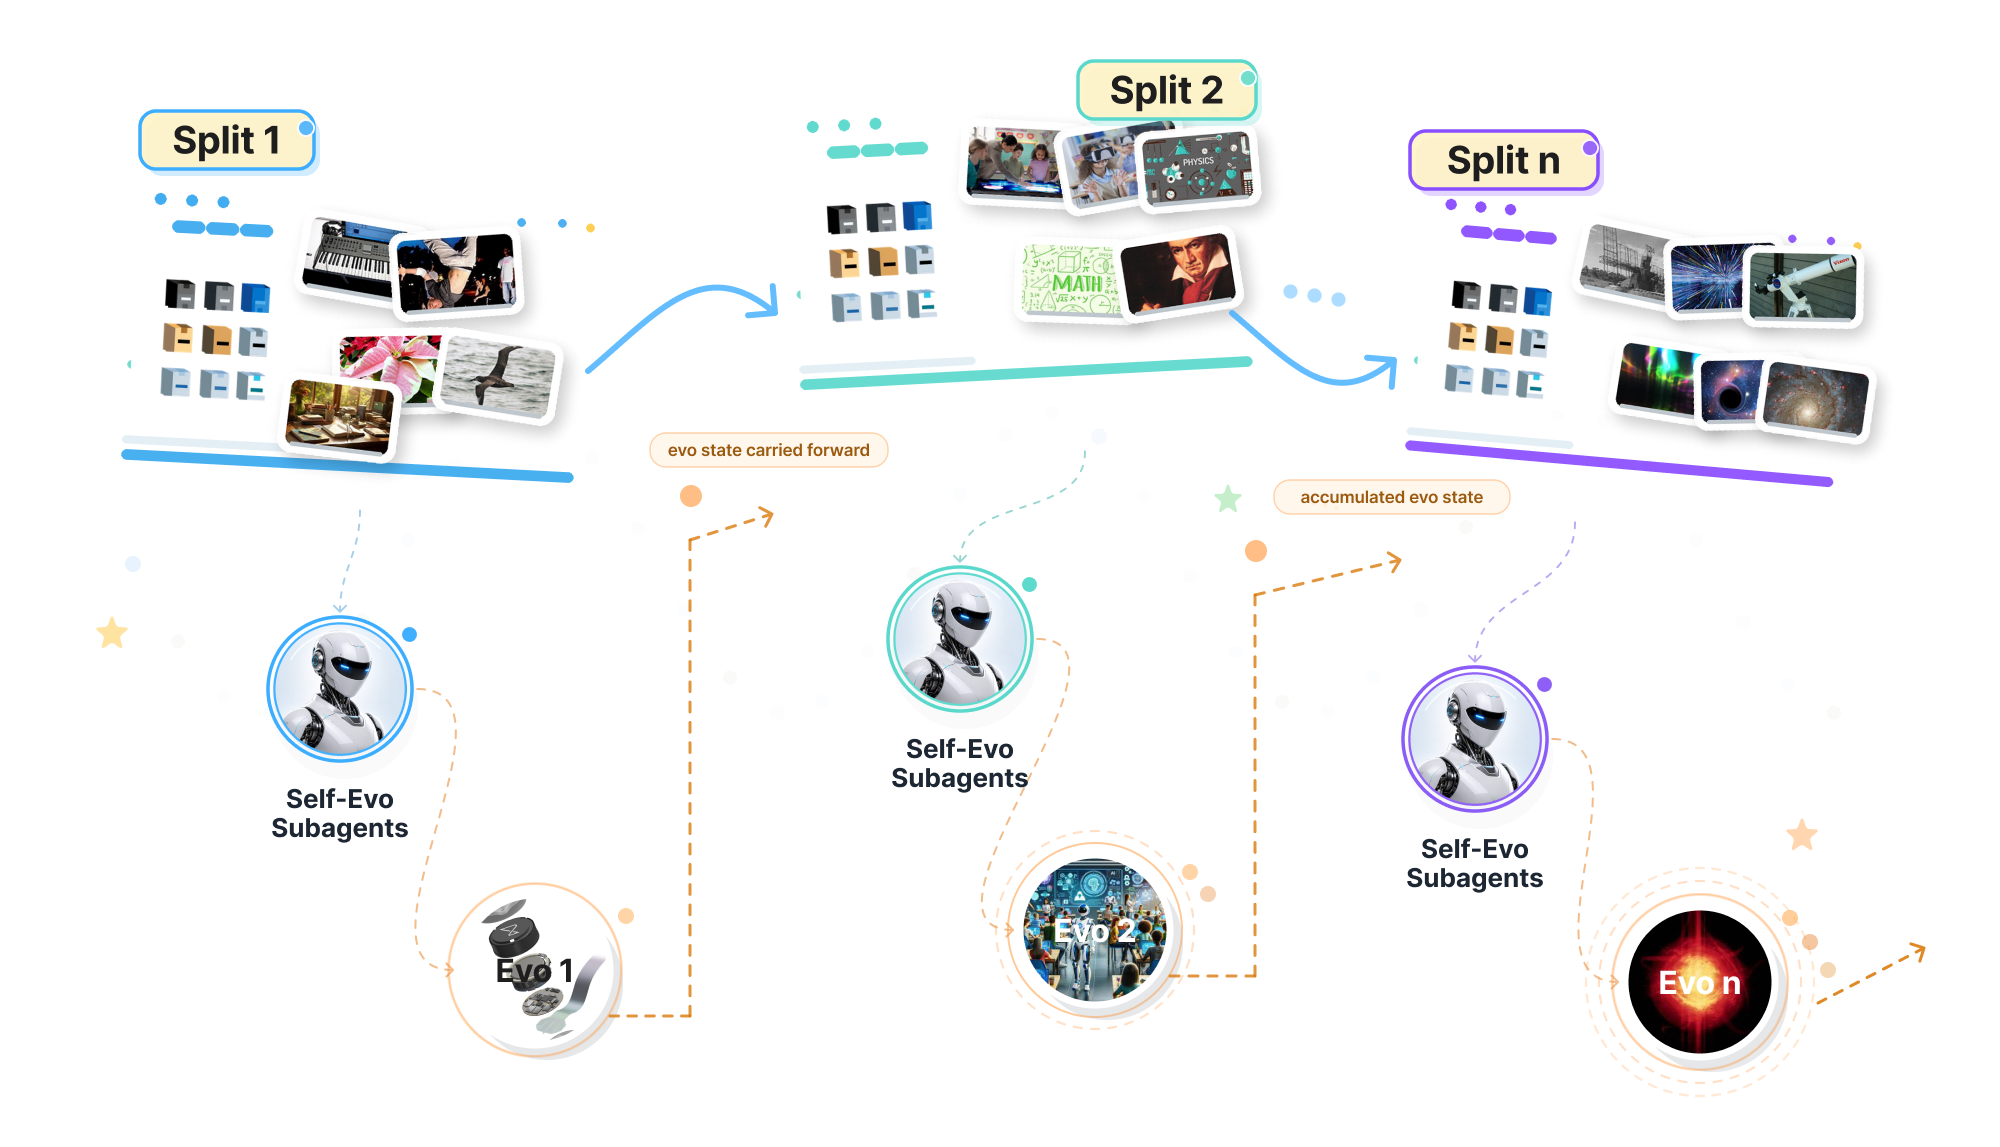
\includegraphics[width=1\linewidth]{figure/lifelong1.png}
    \caption{
    Lifelong memory self-evolution across sequential splits.
    Each split uses only evo-assets promoted from previous splits; failures from the current split are diagnosed and gated after evaluation, and accepted assets are used only by later splits.
    }
    \label{fig:lifelong_selfevo_protocol}
\end{figure}

This subsection focuses on the effect of failure-driven lifelong self-evolution, complementing the dataset-specific static memory results.
The self-evolving variant uses the same memory graph schema, the same base hybrid graph retriever, and the same base writer--answerer configuration as the corresponding static run.
The only difference is that later splits can load evo-assets promoted from earlier splits, such as writer rules, evidence-selection preferences, answerer calibration rules, frame-selection policies, or temporal-normalization policies.







\begin{figure*}[!t]
    \centering
    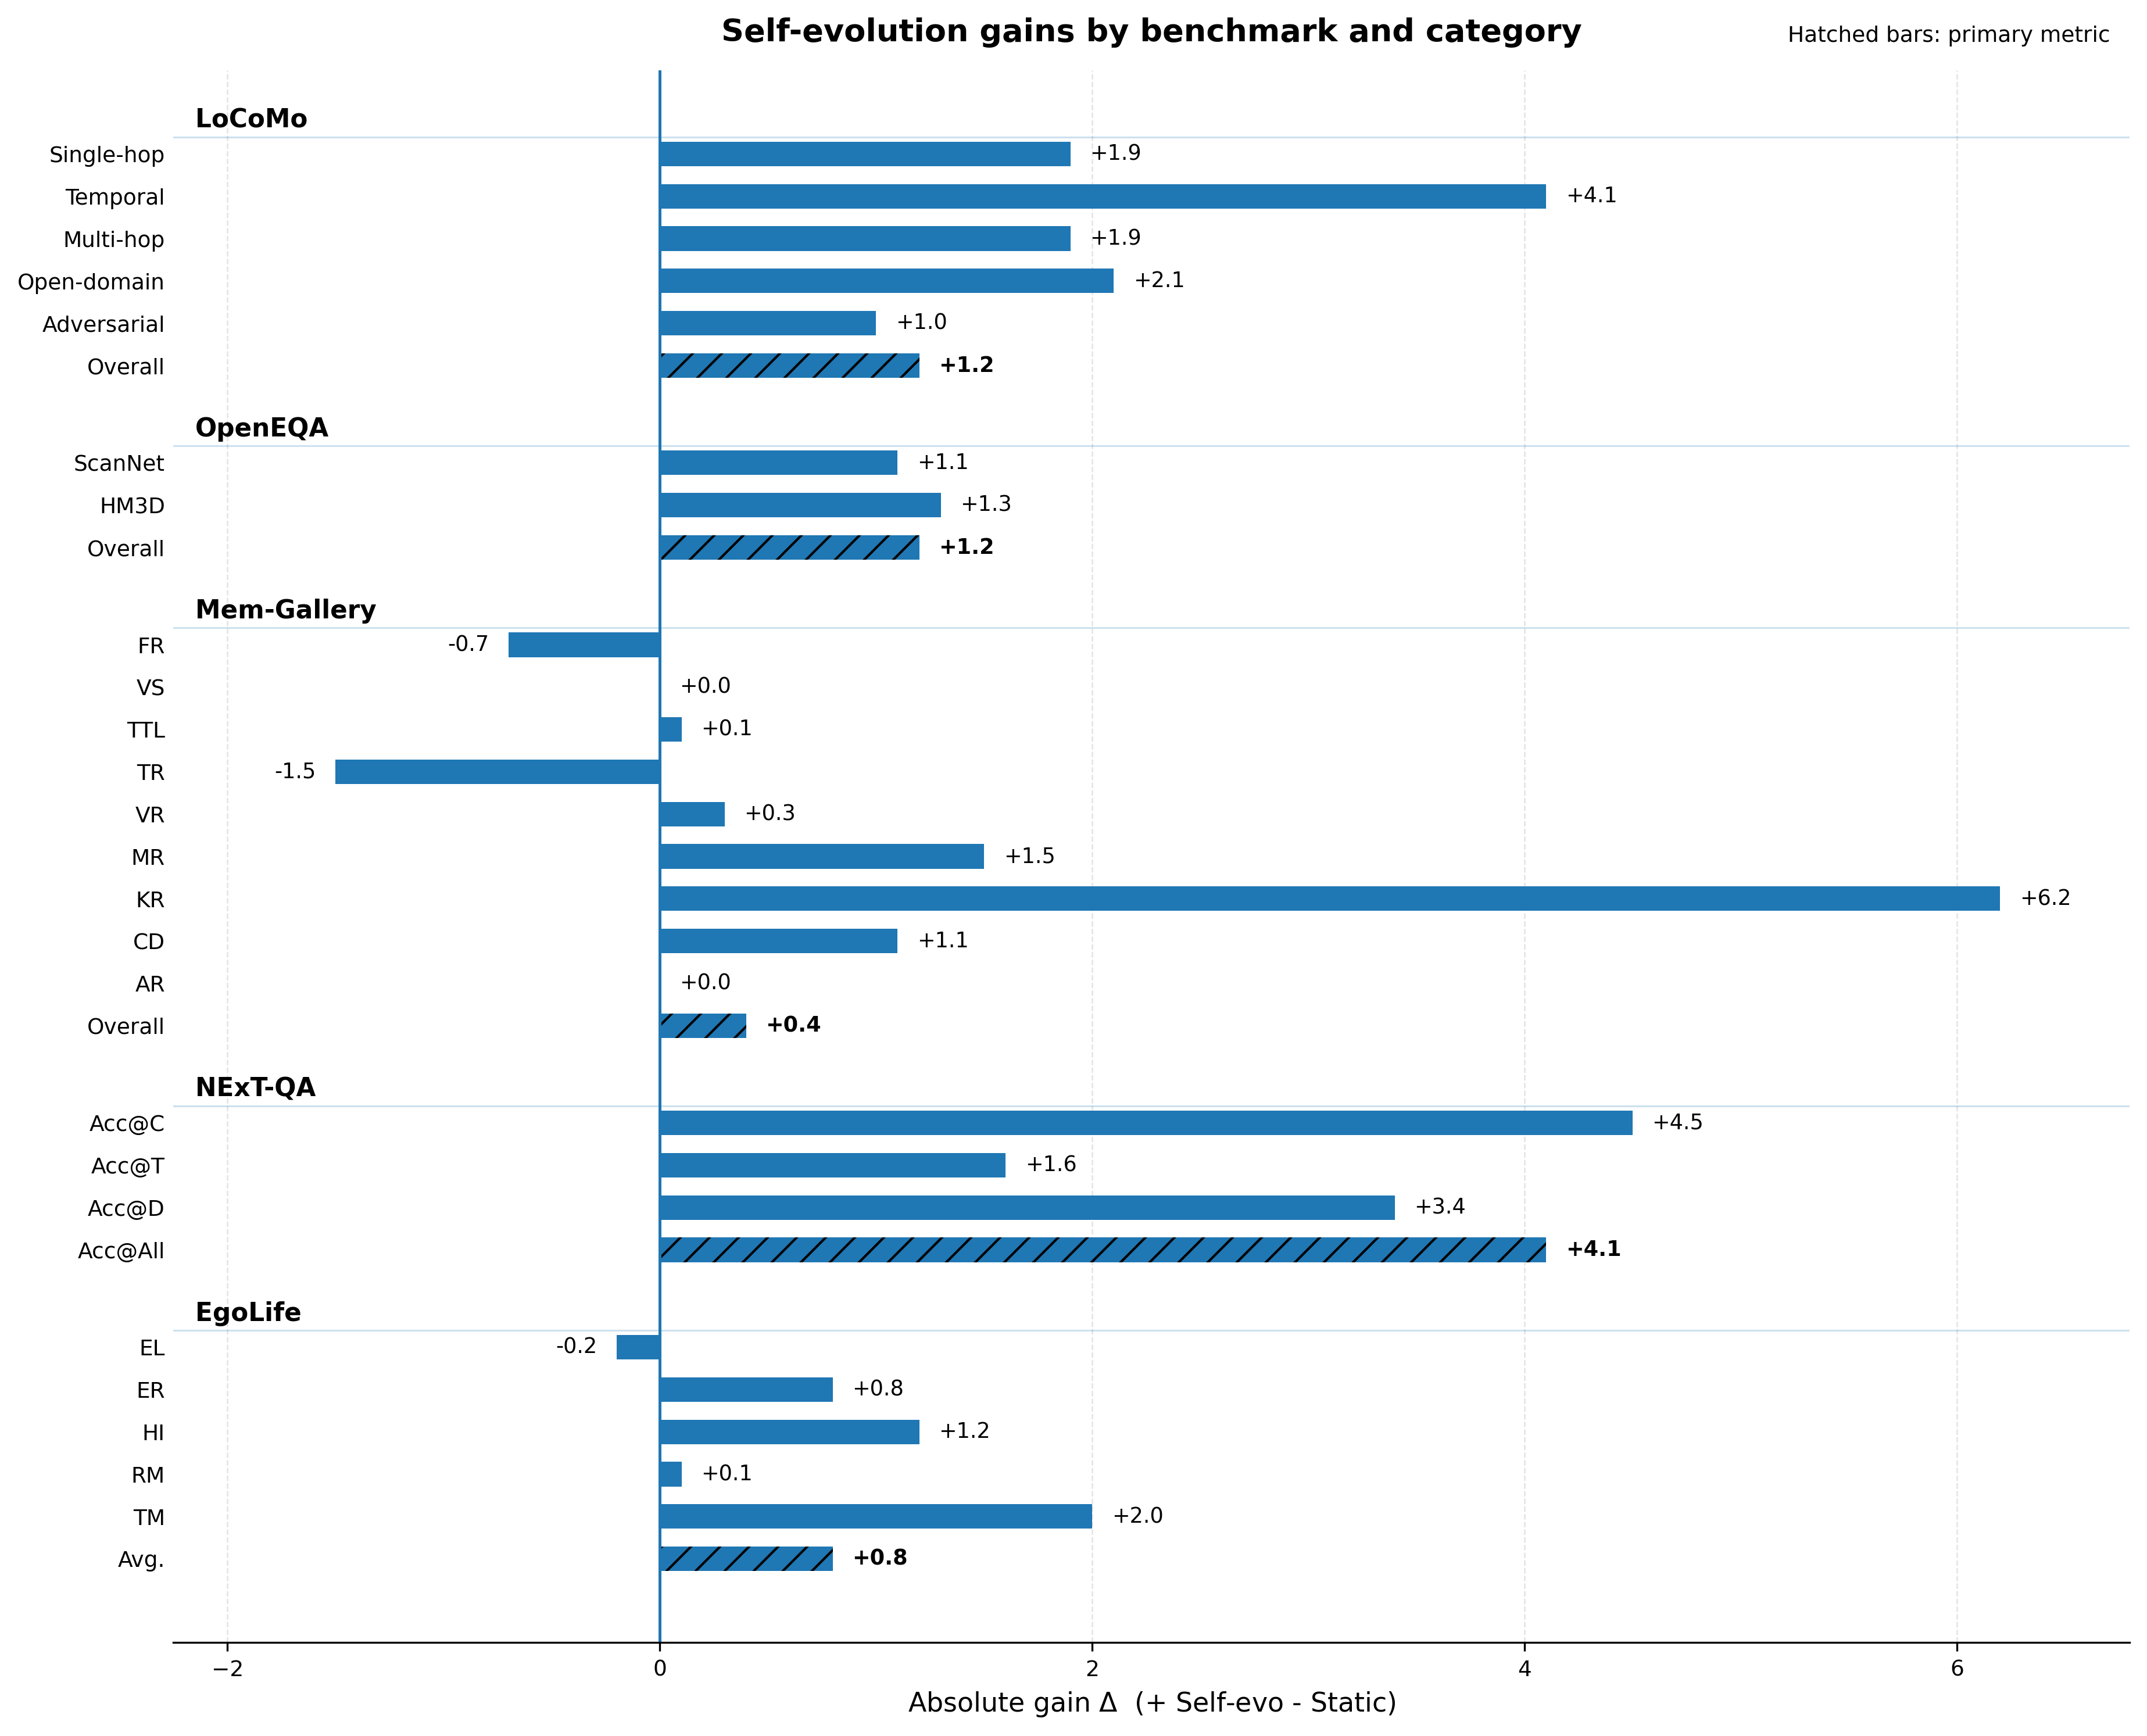
\includegraphics[width=\textwidth]{figure/gain.png}
    \caption{
    Self-evolution gains by benchmark and category.
    Bars show absolute score changes from Static to + Self-evo; hatched bars indicate the primary metric for each benchmark.
    }
    \label{fig:memory-selfevo-gains}
\end{figure*}



Because these experiments are conducted in EQA and QA benchmark settings, the self-evolution loop needs ground-truth answers as a post-hoc correctness signal for diagnosing failures.
This ground-truth signal is used only after a split has already been evaluated.
It is not available during inference, is not written into the memory graph, and does not generate assets for the same split.
This is analogous to how a deployed embodied agent would use interaction feedback in the real world: a user may correct a wrong answer, confirm a right answer, or provide follow-up evidence, and the environment itself may reveal task success or failure through state changes, observations, or execution outcomes.
Thus, the benchmark protocol is a controlled substitute for natural embodied feedback rather than a ground-truth leakage channel.

As illustrated in Figure~\ref{fig:lifelong_selfevo_protocol}, each dataset is partitioned into an ordered sequence of disjoint splits
$\mathcal{D}_1,\ldots,\mathcal{D}_T$.
At evaluation split $t$, the self-evolving variant uses only evo-assets promoted from previous splits, denoted $A_{<t}$.
Failure traces from split $t$ are processed only after evaluation on that split is complete, and the resulting assets can only affect later splits:
\begin{align}
    \mathcal{T}_t, G_t
    &= \operatorname{Run}(\mathcal{D}_t; G_{t-1}, A_{<t}), \\
    \Delta A_t
    &= \operatorname{Gate}\!\left(
        \operatorname{Compile}\!\left(
        \operatorname{Propose}\!\left(
        \operatorname{Diagnose}(\mathcal{T}_t)
        \right)\right)\right), \\
    A_{\leq t}
    &= A_{<t} \cup \Delta A_t .
    \label{eq:memory_eval_self_evo_update}
\end{align}
Here $G_t$ is the updated memory graph and $\mathcal{T}_t$ denotes the recorded answer traces and failure traces.
Only $A_{\leq t}$ is available for later splits.


Figure~\ref{fig:memory-selfevo-gains} visualizes the effect of self-evolution by dataset and category.
Across all five benchmarks, self-evolution improves the primary score over the static memory system.
The largest absolute gain appears on NExT-QA, where Acc@All improves by $4.1$ points.
LoCoMo and OpenEQA both improve by $1.2$ points.
Mem-Gallery shows a smaller overall gain of $0.4$ points, but the category-level gains highlight targeted improvements on knowledge resolution, conflict detection, and multi-entity reasoning.
EgoLife improves from $65.4$ to $66.2$ average accuracy, with the largest category-level gain on TaskMaster.


\FloatBarrier

\subsubsection{Discussion}
\label{subsubsec:memory-discussion}

The per-dataset results show that ABot-AgentOS is strongest when a question requires structured evidence rather than a single visual or textual snippet.
On LoCoMo, the static memory graph reaches near-human overall performance and improves over strong conversational memory baselines, suggesting that source-grounded events, temporal links, and provenance-aware retrieval help long-session recall.
On OpenEQA, the memory system improves over the listed scene-memory baselines under an 8-frame budget, showing that compact graph memories can provide useful spatial and semantic grounding even when visual context is limited.
On Mem-Gallery, ABot-AgentOS Static outperforms the listed memory systems overall and is especially competitive on reasoning, conflict detection, and refusal categories, where provenance and multi-modal relation tracking are important.
On NExT-QA, ABot-AgentOS improves over previous memory-based video agents, indicating that typed event and relation memories are useful for causal and temporal video QA.
On EgoLife, the system achieves the strongest average score while using only one retrieved frame, suggesting that the memory retriever can compress long egocentric streams into highly selective evidence.

The self-evolution results in Section~\ref{subsubsec:memory-selfevo} further show that the memory pipeline can improve without changing the base retriever or leaking current-split answers.
The most consistent gains appear in categories that expose systematic pipeline errors: temporal normalization in LoCoMo, embodied scene disambiguation in OpenEQA, relation and conflict handling in Mem-Gallery, and causal-temporal reasoning in NExT-QA.
Because assets are promoted only after gated validation and are used only on later splits, positive gains indicate reusable memory-pipeline improvements rather than post-hoc repair of the current evaluation split.
The same mechanism is directly compatible with real embodied deployment: instead of benchmark ground truth, the agent can use environmental outcomes and human interaction feedback as the correctness signal for future self-evolution.